\documentclass{article}
\usepackage{amsmath}
\usepackage{amsfonts}
\usepackage{amssymb}
\usepackage[margin=1cm, bottom=2cm]{geometry}
\usepackage{fancyvrb}
\usepackage{svg}
\usepackage{graphicx}
\usepackage{listings}
\usepackage{float}

\newcommand{\drawline}{\vspace{1em}\hrulefill\vspace{1em}}

\begin{document}
\Large

\drawline
\begin{center}
\Large \textbf{Problema 1}
\end{center}

La secuencia de Fibonacci es una serie matemática donde cada número es la suma de los dos números anteriores.

\bigskip

La secuencia comienza con $0$ y $1$, y cada número consecutivo se calcula sumando los dos anteriores.
Los primeros números de la secuencia son: $0$, $1$, $1$, $2$, $3$, $5$, $8$, $13$, \ldots

\bigskip

\underline{Calcule el valor exacto del término número 32 de la secuencia de Fibonacci.}


\drawline
\newpage
\drawline
\begin{center}
\Large \textbf{Problema 2}
\end{center}

\[
\text{Si: }
\begin{cases} 
    a \times a = 27 & \text{y} \\
    a \times b = 9
\end{cases}
\]

\underline{¿Cuánto vale $b \times b$?}


\drawline
\newpage
\drawline
\begin{center}
\Large \textbf{Problema 3}
\end{center}

Hay $N$ puertas en fila, todas cerradas. Una persona camina por las puertas y altera cada puerta (la abre si está cerrada, y la cierra si estaba abierta). En su segunda pasada altera cada 2da puerta, en su tercera pasada altera 3ra puerta, y así consecutivamente, haciendo un total de $N$ pasadas.

\bigskip

Por ejemplo, si $N = 9$, las puertas quedan así:

\bigskip

\begin{verbatim}
Número de puerta: 1 2 3 4 5 6 7 8 9
Estado inicial:   0 0 0 0 0 0 0 0 0 (0 := cerrada, 1 := abierta)
1° pasada:        1 1 1 1 1 1 1 1 1 
2° pasada:        1 0 1 0 1 0 1 0 1 (2°, 4°, 6° y 8° puertas modificadas)
3° pasada:        1 0 0 0 1 1 1 0 0 (3°, 6° y 9° puertas modificadas)
4° pasada:        1 0 0 1 1 1 1 1 0 (4°, 8° puertas modificadas)
5° pasada:        1 0 0 1 0 1 1 1 0 (5° puerta modificada)
6° pasada:        1 0 0 1 0 0 1 1 0 (6° puerta modificada)
7° pasada:        1 0 0 1 0 0 0 1 0 (7° puerta modificada)
8° pasada:        1 0 0 1 0 0 0 0 0 (8° puerta modificada)
9° pasada:        1 0 0 1 0 0 0 0 1 (9° puerta modificada)
\end{verbatim}

\bigskip

En este caso, al final permanecen 3 puertas abiertas.

\bigskip

\underline{Si $N = 2025$, ¿cuántas puertas quedan abiertas al final del proceso?}


\drawline
\newpage
\drawline
\begin{center}
\Large \textbf{Problema 4}
\end{center}

Una diagonal en un polígono regular es cualquier segmento de línea que conecta dos vértices no adyacentes del polígono.
En otras palabras, es una línea recta que une dos esquinas del polígono que no están directamente conectadas por un lado.

\begin{figure}[H]
    \centering
    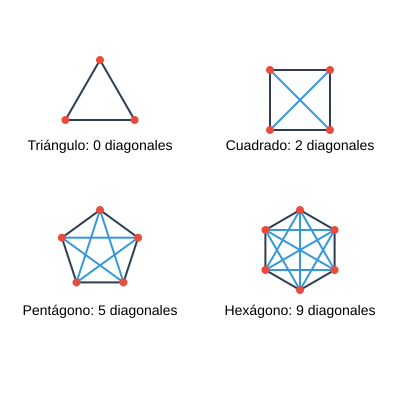
\includegraphics[width=0.5\textwidth]{diagonales.png}
\end{figure}

\underline{¿Cuántas diagonales tiene un polígono regular de $2025$ lados?}


\drawline
\newpage
\drawline
\begin{center}
\Large \textbf{Problema 5}
\end{center}

\bigskip

Una fábrica produce dos tipos de productos. Llamemos $x$ al número de productos del primero tipo que se produce, y llamemos $y$ al número de productos del segundo tipo producidos.

\bigskip
La fábrica está sujeta a varias restricciones:
\begin{itemize}
    \item $(y - x) \le 5$
    \item $x + 6y \le 140$
    \item $4x + y \le 120$
\end{itemize}

\underline{Cuál es la máxima cantidad de productos que puede producir?} \\
\underline{Indique cuánto se produciría de cada tipo de producto.}


\drawline
\newpage
\drawline
\begin{center}
\Large \textbf{Problema 6}
\end{center}

Un cuadrado perfecto es un número que se puede expresar como el cuadrado de un entero. Por ejemplo, 16 es un cuadrado porque $16 = 4 \times 4$.

\bigskip
Nos interesa, dado un conjunto de números, ordenarlos de tal manera que la suma de cada dos números consecutivos sea un cuadrado perfecto.
Por ejemplo, si el conjunto es $\{2, 7, 9, 14\}$, un órden válido sería $[9, 7, 2, 14]$, ya que:
\begin{itemize}
    \item $9 + 7 = 16 = 4 \times 4$
    \item $7 + 2 = 9 = 3 \times 3$
    \item $2 + 14 = 16 = 4 \times 4$
\end{itemize}

\underline{Dar un orden del conjunto $\{1, 3, 6, 8, 10, 13, 15\}$,} \\
\underline{tal que la suma de cada dos números consecutivos sea un cuadrado perfecto.}


\drawline
\newpage
\drawline
\begin{center}
\Large \textbf{Problema 7}
\end{center}

Supongamos que tengo tres premios: premio A, premio B y premio C.
Premio A es el mejor de todos, premio C es el peor de todos, y premio B está en el medio.

\bigskip

Vos tenés que hacer una afirmación - es decir, tenés que decir algo que, o bien es correcto, o bien es falso.
Si tu afirmación resulta ser correcta, te voy a dar alguno de los premios A o B. Si tu afirmación resulta ser falsa, te doy el premio C.

\bigskip


Por ejemplo, si decís "$2 + 2 = 4$", podría darte el premio A, o podría darte el premio B - pero no puedo darte el premio C. Si decís "$2 + 2 = 5$", estoy obligado a darte el premio C.

\bigskip

Supongamos que sos ambicioso y no te vas a ir sin el premio A.

\underline{Escribí una afirmación que me obligue a darte el premio A.}


\drawline
\newpage
\drawline
\begin{center}
\Large \textbf{Problema 8}
\end{center}

Comenzando en la esquina superior izquierda de un tablero de $2 \times 2$, y pudiendo moverse solamente hacia la derecha y hacia abajo,
hay exactamente $6$ rutas hasta la esquina inferior derecha.

\begin{figure}[H]
    \centering
    
\includegraphics[width=0.3\textwidth]{caminos_grilla.png}
\end{figure}

\underline{¿Cuántas rutas de este tipo hay a través de un tablero de $5 \times 5$?}


\drawline
\newpage
\drawline
\begin{center}
\Large \textbf{Problema 9}
\end{center}

Ana y Beto juegan regularmente partidos de ping-pong.
Un partido de ping-pong consiste de una serie de sets, y se juega al mejor 5 sets - el primer jugador en ganar 3 sets gana el partido.
Un set es ganado por el jugador que primero alcanza 4 puntos y tiene una ventaja de al menos 2 puntos sobre su oponente.
Es decir, si ambos jugadores tienen al menos 3 puntos cada uno (conocido como "deuce"), entonces se necesita ganar dos puntos consecutivos para ganar el juego:
uno para obtener ventaja y otro para ganar el set.

\bigskip
Ana y Beto jugaron varios partidos y para cada partido que jugaron anotaron una secuencia de letras, donde 'A' representa un punto ganado por Ana y 'B'
representa un punto ganado por Beto. Luego de jugar varios partidos arman otra secuencia de letras - una 'A' para cada partido ganado por Ana y una 'B' para
cada partido ganado por Beto. Por ejemplo, para tres partidos que jugaron anotaron las siguientes secuencias (agregamos \texttt{()} y \texttt{[]} para indicar
visualmente quién ganó cada set).

\begin{verbatim}
    1° partido: (AAAA)[BBBB](ABAABBAA)(AAABBA)
    2° partido: (BAABAA)[BBBB][ABBBB][BBBAAB]
    3° partido: (BAABABABAA)[ABBABB](BAABABAA)[ABBABABABB](BBAAAA)
    Resultado:  ABA
\end{verbatim}

El resultado es \texttt{ABA} porque los ganadores de los partidos fueron, respectivamente, Ana (ganó 3-1 en sets en el 1° partido),
Beto (ganó 3-1 en sets en el 2° partido) y Ana de nuevo (ganó 3-2 en sets en el 3° partido).

\bigskip

Dados los siguientes partidos jugados:
\begin{verbatim}
    1° partido: BBAAAABBBABBAABABAAABBBBABBABB
    2° partido: BABBAABBABBABABABBABBABABB
    3° partido: AABBBBBAAAAABAABBAAAAABBA
    4° partido: BAABAABAABAABBAAAA
    5° partido: BBBAABBAABABABAABBBBABBABABABB
    Resultado:  ???
\end{verbatim}

\underline{¿Cuál es el resultado final que anotarían?}

% Sets de ejemplo:

% Gana Ana:
% AAAA       (4-0)
% AAABA      (4-1)
% BAAAA      (4-1)
% AAABBA     (4-2)
% BBAAAA     (4-2)
% BAABAA     (4-2)
% ABAABBAA   (5-3)
% BAABABAA   (5-3)
% BAABABABAA (6-4)

% Gana Beto:
% BBBB       (4-0)
% BBBAB      (4-1)
% ABBBB      (4-1)
% BBBAAB     (4-2)
% AABBBB     (4-2)
% ABBABB     (4-2)
% BABBAABB   (5-3)
% ABBABABB   (5-3)
% ABBABABABB (6-4)
\drawline

\end{document}
